\documentclass[../main]{subfiles}

\begin{document}

\chapter{Introduction}\label{ch:introduction}

Learning to program is hard, and students consequently regard programming courses as difficult~\autocite{robinsLearningTeachingProgramming2003,simoesNatureProgrammingExercises2020}.
It is generally accepted that gaining a deep understanding of programming requires experience and feedback~\autocite{gomesEnvironmentImproveProgramming2007}.
This feedback is what makes teaching programming difficult: it is a time-consuming task to provide good and timely feedback on code, especially if the number of students in a course is high~\autocite{zavalaUseSemanticbasedAIG2018,staubitzRepositoryOpenAutogradable2017,queirosPexilProgrammingExercises2011,pirttinenCrowdsourcingProgrammingAssignments2018,gulwaniFeedbackGenerationPerformance2014,tangDatadrivenTestCase2016}.

\section{Origins and use of automated assessment in computer science education}\label{sec:automated-assessment-in-computer-science-education}

Education of concepts that we would now consider computer science goes back as early as the 1940s.
A good overview on the history of computer science education is given in \textcite{tedreChangingAimsComputing2018}, to which we point the reader for a complete overview.
Of particular interest to this dissertation is the education of programming, which began appearing curricula during the early 1960s~\autocite{simonEmergenceComputingEducation2015}.
This is a bit after computer science became recognized as its own scientific discipline in the 1950s and 1960s~\autocite{hopcroftComputerScienceEmergence1987,atchisonComputerScienceNew1971,gornComputerInformationSciences1963,knuthComputerScienceIts1974,denningScienceComputerScience2013}.

From the start of programming education, the need for automated assessment was noted.
Generally considered to be the first publication on automated assessment, \textcite{hollingsworthAutomaticGradersProgramming1960} details their testing framework and remarks that they could not accommodate the number of students in their programming classes without their ``automatic grader''.
Since then, there has been a long history of using automated assessment~\autocite{ala-mutkaSurveyAutomatedAssessment2005,douceAutomaticTestbasedAssessment2005,ihantolaReviewRecentSystems2010,paivaAutomatedAssessmentComputer2022,combefisAutomatedCodeAssessment2022,nayakAutomatedAssessmentTools2022,messerAutomatedGradingFeedback2024}.

In its most basic form, automated assessment for programming exercises translates to using some (educational) software testing framework that will evaluate the submitted code (the submission).
The testing framework determines if a particular submission is correct, based on a set of tests (the test suite) provided by the educators who created the programming exercise.
The result of this evaluation is the feedback given to the students.

There is a significant overlap between the software testing frameworks used in programming education and the ones used in programming contests, where these frameworks are called (online) judges, a term introduced by \textcite{kurniaOnlineJudge2001}.
The International Collegiate Programming Contest (ICPC) is considered to be the oldest and most widely known programming contest.
It traces its roots back to the First Annual Texas Collegiate Programming Championship, held in 1970 at Texas A\&M University.
From 1977 until 2017, the contest was held under the auspices of the Association for Computing Machinery, and known as ACM-ICPC~\autocite{ICPCFactSheet2023}.

In essence, a testing framework used in educational practice or a competition must do the same: evaluate a submission for correctness.
It is therefore not a surprise that judges are heavily used for educational contexts~\autocite{wasikSurveyOnlineJudge2018,zinovievaUseOnlineCoding2021,liuWhoJudgesJudge2023}.
The differences are mostly found in the focus of the testing frameworks.
In educational settings, evaluating the correctness of a submission itself is not the main goal.
The goal is to provide students with formative feedback.
Even more, correctness as the only feedback might not help students in the learning process~\autocite{haoUnderstandingEffectiveDesign2021}.
In a programming contest, the result of an evaluation is often limited to a binary correctness decision: the submission is accepted or rejected.
A second difference is the focus on performance: in general, in an educational setting the focus is on the performance of generating the feedback, while in a competition the focus lies on the performance of the submission.
For example, in some programming contests, a correct submission is expected, but the competition lies in having the fastest submission.

Another area of interest is the practice of software testing in the software engineering field.
As with educational software testing, the essential purpose of software testing is correctness~\autocite{panSoftwareTesting1999}.
The desired or correct behaviours are specified as the functional requirements of the program and say how a program must behave~\autocite{bassSoftwareArchitecturePractice2021}.
Other software quality factors (the non‐functional requirements) that may be tested are its functionality (reliability, usability, integrity), engineering (efficiency, testability, documentation, structure) and adaptability (flexibility, reusability, maintainability)~\autocite{hetzelCompleteGuideSoftware1988}.

What makes educational software testing different is that each programming exercise has a fixed specification, against which multiple submissions must be evaluated~\autocite{wilcoxTestingStrategiesAutomated2016}.
Submissions are usually small to moderate in size, with all source code contained in a single file in most cases.
While educational software testing also evaluates submissions for correctness, correctness itself is not the main goal.
Instead, the goal is to provide formative feedback (or a grade) to the students~\autocite{caizaProgrammingAssignmentsAutomatic2013}.

\section{The Dodona platform}\label{sec:dodona}

As mentioned in the previous section, providing good and timely feedback to students in programming courses almost necessitates a form of automation.
This is no different in our department.
This was initially done (since 2011) using the Sphere Online Judge (SPOJ; \cite{kosowskiApplicationOnlineJudge2008}), which was relatively unique in the fact that it allowed teachers to create their own courses, exercises, and even testing frameworks.
However, the platform targets the organization of programming contests and lacks support for features we wanted to introduce in our programming classes.

\marginnote{As a student, I was one of the last years to uses SPOJ, even if that statement does make me feel old.}
In 2016, the needs for these classes outgrew the Sphere Online Judge, which led to the creation of our own platform: Dodona~\autocite{vanpetegemDodonaLearnCode2023}.
Dodona is now used by most higher education institutions in Flanders and by many schools providing secondary education.
As of May 2024, Dodona has more than \num{69200} registered users and has evaluated almost 18 million submissions.

Dodona has been developed with support for multiple programming languages from the start.
It has a strict separation between the platform (responsible for managing courses, students, and exercises) and the testing framework (determining if submissions are correct).
This separation has allowed for easily supporting a multitude of programming languages.
Within Dodona, the testing framework is called a judge (and evaluating a submission for correctness is called judging), as it was done in the Sphere Online Judge.

While the earliest Dodona judges targeted Python and JavaScript submissions, its interface for judges proved to be generic enough that it can support a multitude of scenarios.
For example, there are currently judges for C, Haskell, Java, Prolog, R, Scheme, Bash, C\#, JavaScript, and Python (and also TESTed of course).
There are also a few less straightforward judges, such as HTML, SQL, Markdown, and Turtle.

\subsection{Architecture}\label{subsec:architecture}

The separation between the platform itself and the judge is also reflected in the architecture of Dodona.
The platform itself is a fairly standard web application written in Ruby on Rails.
The web application follows the recommendations by Ruby on Rails: it uses a model-view-controller architecture.
Most pages, especially simpler ones, use server-side rendering.
More recently, complex pages have been added that use web components.

Evaluating submissions has some performance and security considerations~\autocite{wasikSurveyOnlineJudge2018}, as a submission is untrusted code that is executed.
Dodona solves this by running the evaluation completely inside a dedicated Docker container~\autocite{pevelerComparingJailedSandboxes2019}.
At a high level, an evaluation of a submission goes through the following process:
\begin{enumerate}[noitemsep]
    \item The submission is saved to the database, and a job is started to perform the evaluation.
    \item A predefined and judge-specific Docker image is used to create a Docker container.
          In this container, all dependencies for the judge are available.
    \item A temporary directory is created by Dodona containing the submission, the test suite for the relevant exercise, and (optionally) additional exercise-specific resources.
    \item This folder is mounted in the container.
    \item The judge runs inside the Docker container, using a well-defined interface containing some metadata for the judge.
    \item During the evaluation, the judge outputs the feedback in a well-defined format on standard output.
    \item The output is captured and saved, after which the feedback is shown to the submitter.
\end{enumerate}

The Docker containers run on a dedicated pool of worker servers.
Using dedicated servers, a misbehaving submission (either accidental, like issues in the submission or bugs in the judge itself, or malicious code) has no effect on the stability of the platform itself.
Using worker servers also allows for easy scaling if the number of submissions increases.

\subsection{Features for educators}\label{subsec:features-for-educators}

Dodona offers a host of features for educators.
For example, it supports a sophisticated course and user management system.
Educators can create dedicated courses on Dodona to reflect courses in real life.
Students can then subscribe to their relevant courses.
A course consists of a number of series, which in turn contain some exercises, which allows for creating learning paths in the course.

Dodona provides detailed statistics and data visualizations of the progress students make in a course and for each series.
Every series can also have a separate deadline, which allows for spreading the workload throughout a semester.

There is a dedicated mode for ``evaluations'' of students, which is a streamlined way to add manual feedback to submissions.
This makes assessment easier.
For example, we use this mode to organize exams.
A hidden series (which is invisible to students) is shared at the start of an exam.
This series contains the exercises that students need to solve in the exam.
After the deadline, Dodona can automatically select the latest submission before the deadline for each student.

Then, educators can anonymously provide feedback and grades (with an educator-provided rubric) on these submissions.
During the evaluation, the feedback of the automated assessment is also available to aid the educators.
After all submissions have been processed, educators can release the feedback to the students, who can then view the feedback and grade they received.

\subsection{The feedback table}\label{subsec:the-feedback-table}

\begin{figure}
    \begin{wide}
        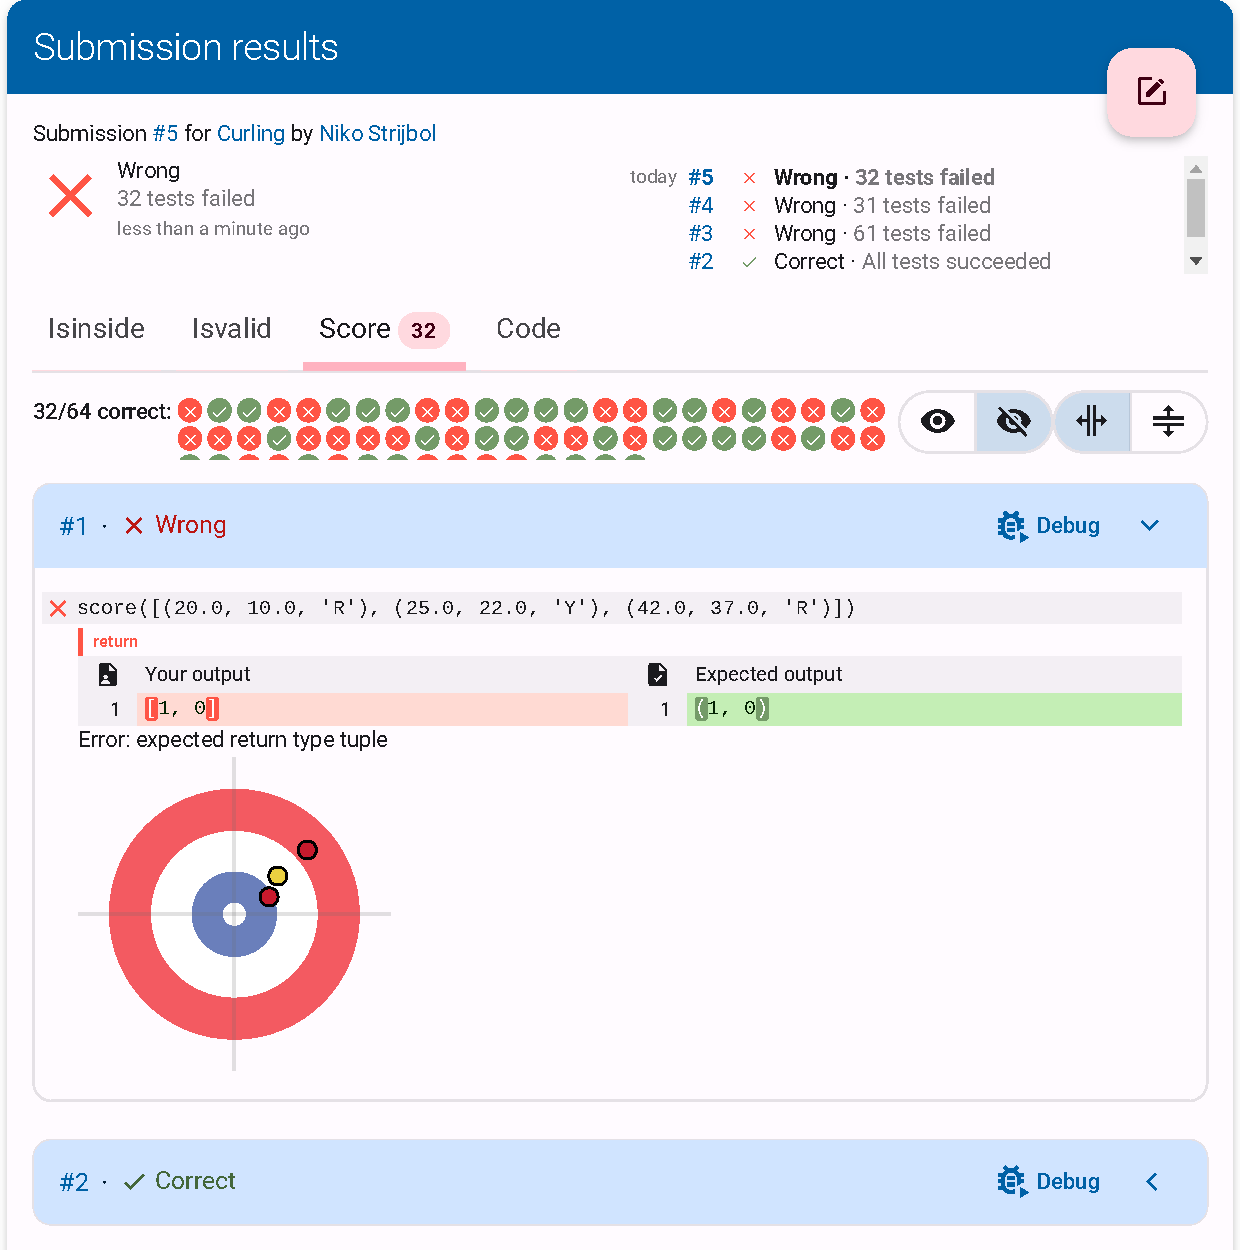
\includegraphics[width=\linewidth]{curling}
    \end{wide}
    \caption{
        An example of the feedback table for an incorrect Python submission for the exercise \textit{Curling} on Dodona.
        The feedback is split into three tabs (the fourth tab, ``Code'', contains the submission itself).
        As can be seen below the tabs, only 32 of the 64 test cases are correct.
        The figure show the first two test cases, the first of which is incorrect: the function should have returned a tuple, but returned a list instead.
        Besides showing the difference between the expected and actual value, Dodona also allows showing more information.
        In this case, a visual rendering of the curling position is given to aid students in debugging their code.
    }
    \label{fig:curling-feedback-table}
\end{figure}

One of the most important elements for both students and educators is the feedback table (\cref{fig:curling-feedback-table}).
This feedback table is flexible enough to accommodate a wide variety of feedback.
In the example, three types of feedback are illustrated: the difference between the expected and generated return value, a custom message, and an image.

As the feedback table shows custom data from an exercise or judge, which are not necessarily trusted, special attention has been paid to make the feedback table secure.
For example, all content is rigorously sanitized to prevent cross-site scripting attacks~\autocite{guptaCrossSiteScriptingXSS2017}.

\subsection{Exercises and content management}\label{subsec:exercises-and-content-management}

Dodona currently supports two types of ``learning activities'': programming exercises and reading activities.
A reading activity requires no submission, but students can mark them as read to confirm they did the reading.
Programming exercises allow students to submit code and receive feedback on their submissions.
However, the bar for what constitutes code can be low.
For example, Dodona has a Markdown judge, which generates a rendered (HTML) version of the Markdown code submitted by students, without actually evaluating anything more than the validity of the Markdown.
Dodona can thus be used to collect plain text submissions from students.

Exercises in Dodona are managed in Git repositories.
A repository with a well-defined structure\footnote{\url{https://docs.dodona.be/en/references/repository-directory-structure/}} is usable as the source for exercises in Dodona.
This allows educators to be the owners of their exercises, in addition to all the other benefits of version control.
Every time an exercise is updated in the repository, Dodona will synchronize the exercises on the platform with the exercises in the repository.

A programming exercise consists of a few different parts.
Besides a test suite, which is needed for automated feedback, exercises also need a problem statement that specifies what students should do.
In Dodona, a problem statement is a Markdown of HTML file, in which educators have free rein (within limits due to security considerations) to describe their exercise.
The programming exercise (including a problem statement and test suite), together with a judge (the Docker image and the testing framework) form a \emph{task package} as defined by \textcite{verhoeffProgrammingTaskPackages2008}.

\section{Structure of this dissertation}\label{sec:a-note-on-the-structure-of-this-thesis}

The root motivation for every part of this dissertation is the observation that there exists a gap in existing educational tools, often with Dodona as a starting point.
We then set out to propose tools that fill this gap.
More concretely, we can define four main research questions, which this dissertation addresses:

\begin{description}
    \item[RQ1] Can we design an educational software testing framework that supports automated assessment across programming languages based on a single test suite?
    \item[RQ2] What is the most ergonomic way to author programming exercises with support for automated assessment across programming languages?
    \item[RQ3] Can we design an educational software testing framework for the block-based programming language Scratch?
    \item[RQ4] Can we design an (educational) debugger for the block-based programming language Scratch?
\end{description}

While we did not intend to split the textual and block-based tools initially, it quickly became clear that the needs for both, in addition to the existing research, were different enough to warrant a separate approach.
This is reflected in this dissertation: the first part (\cref{ch:tested1,ch:tested-dsl}) is about textual programming languages, TESTed and TESTed-DSL\@.
It discusses the first two research questions.
The second part (\cref{ch:scratch-the-programming-environment,ch:itch,ch:blink,ch:scratch-execution-model}) is about Scratch-related tools (Itch, Poke, Blink, and the Scratch execution model).
It discusses the last two research questions.

Finally, \cref{ch:conclusions-and-opportunities} draws the general conclusions and discusses some future opportunities.
Each chapter also contains a similar section where the details of that specific chapter are discussed.

The remainder of this chapter gives a high-level overview of each part: the context, motivation, and where applicable, our previous publications.
Similar to the conclusions, each chapter also has its own introduction, where the specifics for that chapter are introduced.

\section{The first part: TESTed}\label{sec:intro-tested}

The reason for asking the first research question was inspired by an observation that some duplicate work happened when working with Dodona, both for programming exercises and for judges.

A lot of programming exercises on Dodona are usable in multiple programming languages.
However, to use an exercise in another programming language, first a hard copy of the exercise had to be made.
Then the test suite had to be converted manually to the test suite format used by the judge for that particular language.
The other parts of the exercise (the configuration and problem statement) also needed to be converted manually.
Additionally, since the exercises are copied, the exercises have to be kept in sync manually, or they risk diverging.

Implementing judges for different programming languages was also repetitive.
For each judge, a new test suite format had to be created, and all other tasks that a judge does (e.g.\ test scheduling, output handling) had to be re-implemented for each new judge.
Supporting a new feature also requires doing it for every judge, which often does not happen in practice.

\subsection{Programming-language-agnostic exercises}\label{subsec:programming-language-agnostic-testing}

The answer to the first research question is yes.
Specifically, we created TESTed, an educational software testing framework.
One of its defining features is the ability to create programming-language-agnostic exercises.
This means that the same exercise (with one test suite) can be solved in multiple programming languages, with support for automated assessment.

TESTed is discussed in \cref{ch:tested1}, which is based on \textcite{strijbolTESTedEducationalTesting2023}.
\marginnote{A doctoral dissertation has no page limit, after all.}
Compared to the original publication, the chapter has been expanded with more information about the inner workings of TESTed, in addition to going more in-depth on technical aspects of the framework.

\subsection{Ergonomic authoring of exercises}\label{subsec:ergonomic-testing}

With a working prototype at hand, the second research question came rather naturally.
We took a step back to look at what is required to go from a prototype to a viable option for creating programming exercises.
This analysis aimed to ensure the exercises could be used in educational practice, including high-stakes tests such as exams.
We want TESTed to be suitable for both educators in higher education and secondary education.
Our ambition was to make TESTed the default option for creating programming exercises in Dodona.

The result of this research is presented in the second publication, \textcite{strijbolTESTedDSLDomainspecificLanguage2024}, which is included almost verbatim as \cref{ch:tested-dsl}.
By looking at (educational) software testing more broadly, we find two missing parts of the process of creating programming exercises.
The first missing, but important, part is an ergonomic and approachable way of creating test suites for exercises.
Our solution is TESTed-DSL, a domain-specific language for authoring programming-language-agnostic exercises with support for automated assessment.
The second missing part is support for language-agnostic task descriptions.
We show that TESTed-DSL can also be used for task descriptions.

A new insight while working on TESTed-DSL was that TESTed is not only useful for creating programming-language-independent exercises, but also suitable for exercises that are not intended to be used in multiple programming languages.
Therefore, we have taken special care to design TESTed-DSL to be useful for a wide audience of educators, including higher and secondary education.
For this reason, we also invested in our documentation, which contains reference documentation and a set of tutorials for commonly used exercise types.

\subsection{Organization of the first part}\label{subsec:organization-of-the-first-part}

One consequence of basing the two chapters on publications is that there is some overlap: for example, the introductions in both chapters broadly cover the same topic.
However, the focus of both is different enough that we feel there is no problem: they are not verbatim copies.
Another example of a consequence is the terminology used for the levels in the test suites (\cref{subsec:structure-of-a-test-suite,subsec:dsl-test-suite-structure}), which differs.
The first chapter uses the terminology as used by Dodona, while the second chapter changes the terminology in the DSL to align more closely with the terminology used in the literature.
This illustrates the progressive insight that comes when working on a tool, and the interplay between the design stages and its application in practice.

Research on TESTed was started in 2019 as a master's thesis~\autocite{strijbolTESTedOneJudge2020}.
Similarly, TESTed-DSL also finds its origins in a master's thesis~\autocite{selsTESTedProgrammeertaalonafhankelijkTesten2021}.

\subsection{Repositories and user documentation}\label{subsec:repositories-and-code}

As a software project, the source code for TESTed is important, if not more important than this dissertation.
Both TESTed and TESTed-DSL share the same repository\footnote{\url{https://github.com/dodona-edu/universal-judge}}, which is published under the \textsc{mit} licence.

Two sets of documentation are available, aimed at a different target audience:

\begin{itemize}
    \item The guides for educators wanting to create programming exercises\footnote{\url{https://docs.dodona.be/en/guides/exercises/}}.
    Most of these guides are currently only available in Dutch.
    \item The reference documentation, for a more in-depth look into more technical subjects\footnote{\url{https://docs.dodona.be/en/references/tested/}}.
    For example, this includes the documentation on how to extend TESTed to add support for additional programming languages.
\end{itemize}

\section{The second part: Scratch}\label{sec:the-second-part:-scratch}

For young children, learning to program for young children is often done with specialized programming languages.
The most-used language in this context is Scratch, a visual, block-based programming language~\autocite{resnickScratchProgrammingAll2009}.

Since Dodona is independent of any testing framework, we thus asked the third research question: ``Can we design an educational software testing framework for Scratch?''.
Our intention was to add support for Scratch to Dodona.

\subsection{Testing Scratch code}\label{subsec:testing-scrath-code}

The first prototype of Itch, our testing framework for Scratch, did just that: it added support for evaluating Scratch submissions in Dodona.
However, Scratch is not only a programming language, but a complete programming environment.
We realized that properly supporting Scratch required accommodations that were too different from what Dodona could (or would) provide.
Additionally, while our group had experience with programming exercises for text-based languages, we had much less experience with Scratch in an educational context.

To address these issues, we sought an industrial and commercial partner.
We found this partner in CodeCosmos, the international brand of FTRPRF, which is an educational publisher that creates, among other things, teaching packs.
Schools can use these to fulfil their obligations as part of the move to introduce more computational thinking in secondary education.

The work was divided as follows: Ghent University was responsible for the technical aspects of the automated feedback for Scratch exercises, while CodeCosmos provided the lessons, the educational support, and last but not least, actual students to use the teaching packs.
Readers interested in knowing more might like to read an article about this collaboration in \textit{Dare To Think}, Ghent University's online magazine\footnote{\url{https://www.durfdenken.be/en/research-and-society/coach-codi-boosting-tool-helps-children-become-independent-coders}}.

The testing framework, the answer to the third research question, is described in \cref{ch:itch}.
Itch allows both static and dynamic tests on Scratch exercises, which provides a lot of flexibility to educators.
Especially the dynamic testing allows for exercises that allow (within limits) the exploratory nature of Scratch to remain.

Itch test suites for Scratch exercises are written in JavaScript.
While working with CodeCosmos on creating Scratch exercises, it became clear that the JavaScript test suites were a big hurdle for educators without a computer science background.
As a lot of software testing frameworks are written in the same programming language as the code they test, we also investigated this possibility: ``Can we design an educational software testing framework for Scratch with test suites written in Scratch?''.
The result of this was Poke, a prototype of a testing framework for Scratch with test suites written in Scratch (\cref{sec:poke:-a-testing-framework-written-in-scratch}).
While possible, there are still open questions regarding the practical use of such a framework in an education setting.

\subsection{Debugging Scratch code}\label{subsec:debugging-scratch-code}

The goal of educational software testing and automated assessment is to provide students with feedback on their code.
However, the feedback in itself is not enough: we want students to be able to use that feedback and be able to correct their code if something went wrong.
The next step, after a failed test, is then to debug the submission, which is a two-step process~\autocite{myersArtSoftwareTesting2012}.
Step one is determining the exact nature and location of the error, and step two is fixing said error.

It is well known that determining the cause of an observed failure is challenging~\autocite{ammannIntroductionSoftwareTesting2016}.
The debugging process is difficult, especially for novice programmers~\autocite{mccauleyDebuggingReviewLiterature2008}.
This has led to the creation of various tools to help with this, chief among them the debuggers~\autocite{rosenbergHowDebuggersWork1996}.

This is also the case with text-based languages.
For example, \cref{fig:curling-feedback-table} shows a ``Debug'' button in the feedback table of Dodona.
However, for Scratch, this area is much less developed.
The fourth research question thus became: ``Can we design a debugger for Scratch?''.

\Cref{ch:blink} discusses our answer to this question, in the form of Blink, our time-travelling debugger for Scratch.
A time-travelling debugger allows the programmer to go back in the execution, often by recording program execution~\autocite{barrTardisAffordableTimetravel2014,barrTimetravelDebuggingJavaScript2016,czaplickiAsynchronousFunctionalReactive2013,balzerEXDAMSExtendableDebugging1969,ungarDebuggingExperienceImmediacy1997,chenReversibleDebuggingUsing2001,crescenziReversibleExecutionVisualization2000}.

This chapter is an almost verbatim copy of a publication: \textcite{strijbolBlinkEducationalSoftware2024}.
We took special care to make the debugger intuitive for the young target audience of Scratch.
Initial experiments in the classroom show that children do in fact find the debugger intuitive and useful, particularly stepping through the code and the time travel feature.

\subsection{The Scratch execution model}\label{subsec:the-scratch-execution-model}

While working on the debugger, we also began looking more deeply into the Scratch execution model.
The Scratch execution model combines a fixed-step time loop (30 frames per second) with an almost-cooperative threading model.
This means that threads are seldom interrupted, mostly relying on explicit yielding to other threads.

This threading model was chosen because it minimizes the occurrence of race conditions, although concurrency-related issues still occur~\autocite{maloneyScratchProgrammingLanguage2010}.
The cooperative nature of the threading model also has drawbacks: it can lead to unexpected behaviour when working with multiple sprites.

Additionally, the execution model also limits how a debugger can work, without resorting to deviating from the execution model as used during normal execution.

We therefore propose and investigate some changes to the Scratch execution model in \cref{ch:scratch-execution-model}.
The chapter begins with a detailed look at how the current execution model behaves, followed by our proposed changes.
Since Scratch is so widely used, our changes should not negatively impact existing Scratch programs.
We therefore analyse what a typical Scratch project looks like.
Finally, we benchmark our changes against some representative projects and report on the results.
We conclude that our proposed changes do not cause problems for existing Scratch projects, while still being an improvement for debuggers.

\subsection{Organization of the second part}\label{subsec:organization-of-the-second-part}

The second part starts with a short chapter that introduces Scratch, the programming language and environment: \cref{ch:scratch-the-programming-environment}.
Next, \cref{ch:itch} discusses Itch, our Scratch testing framework.
The next chapter, \cref{ch:blink} discusses Blink, our debugger for Scratch.
Finally, \cref{ch:scratch-execution-model} discusses the Scratch execution model, our proposed changes to it, an analysis of Scratch projects, and an evaluation of our proposed changes.

Work on these various tools for Scratch often began as a master thesis~\autocite{makItchEenEducatief2019,voetenEenBlokgebaseerdTestframework2023,goethalsEenTimeTravelling2023,deproftBlinkEenEducatieve2022}.

\subsection{Repositories and user documentation}\label{subsec:repositories-and-code-scratch}

The source code for Blink\footnote{\url{https://github.com/scratch-ed/blink}} is available under the same licence as Scratch, the \textsc{bsd} 3-Clause ``New'' or ``Revised'' Licence.
We also host an online instance of the debugger\footnote{\url{https://scratch.ugent.be/blink/}}.

\end{document}
